\problemname{Mineral deposits}

\illustration{.3}{img/turnbull.jpg}{Eroding mud face exposing new minerals. Photo: Michael D.\ Turnbull, licencse: CC BY-SA.}

\noindent
One of the major goals of space exploration is extra-terrestial mining. 
As part of this, you are now approaching an astroid. 
Preliminary scans show that $k$ mineral deposits are present on this asteroid, though their precise locations are unkown.

\medskip

The surface of the asteroid can be seen as a grid of integer coordinates.
Each of the mineral deposits is located at unkown integer coordinates such that the $i$th deposit has coordinates $(x_i, y_i)$ with  
$-b \le x_i \le b$ and $-b\le y_i \le b$ %constraint:depositcoords
for some integer $b$ corresponding to the size of your initial scan.

To determine the locations of these mineral deposits, you may send probes to the surface of the asteroid. 
This is a time-consuming process, so the probes can be sent out in waves;
several probes can be sent out at once, minimising the time you have to wait until they arrive at the surface.

Say you sent a wave of $d$ probes to the surface at coordinates $(s_j,t_j)$ for $1\leq j\leq d$.
When a probe arrives at its coordinates it determines the Manhattan distances to each of the $k$ deposits and sends them back to the ship. 
The data packets arrive at the same time, and it is not possible to determine which probes returned which distances. 
Thus the wave returns the $k\cdot d$ integer distances
\[|x_i-s_j| + |y_i - t_j| \qquad\text{for all } i \in \{1,\ldots,k\} \text{ and } j \in\{ 1,\ldots,d\}\,.\]
These distances will be in sorted order.

You need to minimise the number of waves of probes that is sent to the surface.


\subsection*{Interaction}

This is an interactive problem.
Interaction begins with you reading a single line containing three integers $b$, $k$, $w$:
the grid's boundary~$b$,
the number~$k$ of deposits,
and the maximum number~$w$ of waves you may send.

You then ask at most $w$ queries, each corresponding to a wave.
A query consists of \texttt{?} followed by $2d$ integers separated by space, such as ``\texttt{?} $s_1$ $t_1$ $\cdots$ $s_d$ $t_d$'', where the number~$d$ of probes in this wave must satisfy
$1\leq d\leq 10^4$. % constraint:wavesize
The values $(s_i,t_i)$ are interpreted as the coordinates of the $i$th probe and must satisfy
$-10^8 \leq s_i \leq 10^8$ and $-10^8 \leq t_i \leq 10^8$. % constraint:probecoordinates
The response is a single line with $k \cdot d$ integers in sorted order, all pairs of Manhattan distances between the hidden deposits and the probe coordinates.
Interaction ends with you printing a single line consisting of \texttt{!} followed by $k$ points $x_1, y_1, x_2, y_2, \ldots x_k, y_k$, separated by space.
This must be your last line of output.

Your submission is considered correct if you print all locations of the deposits.
You may print them in any order.

\subsection*{Constraints and scoring}

We always have 
$1\leq b \leq 10^8$ % constraint:b
$1 \leq k \leq 30$, % constraint:k
and
$2 \le w \le 10^4$. % constraint:w

Your solution will be tested on a set of test groups, each worth a number of points.
Each test group contains a set of test cases.
To get the points for a test group you need to solve all test cases in the test group.
Your final score will be the maximum score of a single submission.

\medskip
\begin{tabular}{lll}
Group & Points & Constraints \\\hline
  $1$ & $9$ & $k = 1, w = 10^4$\\
  $2$ & $19$ & $w \ge 500$\\
  $3$ & $11$ & $w \ge 210$\\
  $4$ & $7$ & $w \ge 130$\\
  $5$ & $20$ & $w \ge 3$, $b \le 10^4$\\
  $6$ & $15$ & $w \ge 3$, $b \le 10^7$\\
  $7$ & $19$ & $w \ge 2$
\end{tabular}

\subsection*{Example}

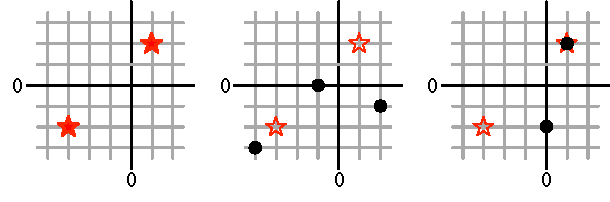
\includegraphics[width=.6\textwidth]{img/sample1.pdf}

In this example, there are $k=2$ mineral deposits at positions $(1,2)$ and $(-3,-2)$, shown as red stars.
In the first wave, you might send $d=3$ probes to $(-4,-3)$, $(-1, 0)$, and $(2,-1)$, shown as black dots.
This wave would return the $6$ distances \[
  2, 4, 4, 4, 6, 8\,.
\]
In the next wave, you might send $d=2$ probes to $(1,2)$ and $(0,-2)$.
This wave would return the $4$ distances \[
  0, 3, 5, 8\,.
\]
The sample interaction below ends with a correct answer to the position of the two mineral deposits.
The example is only meant to demonstrate the output format; no indication of how to solve this problem is implied.
